\documentclass[conference]{IEEEtran}
\IEEEoverridecommandlockouts
\usepackage{cite}
\usepackage{amsmath,amssymb,amsfonts}
\usepackage{algorithmic}
\usepackage{graphicx}
\usepackage{textcomp}
\usepackage{float}
\usepackage{xcolor}
\usepackage{seqsplit}
\usepackage[hidelinks]{hyperref}
\usepackage{lipsum} 

\def\BibTeX{{\rm B\kern-.05em{\sc i\kern-.025em b}\kern-.08em
    T\kern-.1667em\lower.7ex\hbox{E}\kern-.125emX}}
\begin{document}

\title{Computer (or machine?) Vision - Emotion Recognition in
Passengers of Autonomous Vehicles}

\author{\IEEEauthorblockN{Samed Voßberg}
    \IEEEauthorblockA{\textit{Information Systems (1953862)} \\
        \textit{Karlsruhe Institute of Technology (KIT)}\\
        urgfl@student.kit.edu}
    \and
    \IEEEauthorblockN{Niklas Wagner}
    \IEEEauthorblockA{\textit{Systems Engineering (2495996)} \\
        \textit{Karlsruhe Institute of Technology (KIT)}\\
        uvssk@student.kit.edu}
    \and
    \IEEEauthorblockN{Felix Mätzler}
    \IEEEauthorblockA{\textit{Systems Engineering (2495689)} \\
        \textit{Karlsruhe Institute of Technology (KIT)}\\
        uvian@student.kit.edu}
}
\maketitle

\begin{abstract}
    \lipsum[2-4]
\end{abstract}

\begin{IEEEkeywords}
    Autonomous driving, User experience, Emotion recognition
\end{IEEEkeywords}

\section{Introduction}
 - Why valence and arousal are important? \\
 - Constraint: Our model can't handle two much parameters?\\
 - Datasets are (obviously) not similar \\
 - Some stats about state of the art models which are still not really good \\
 
Test Ciation \cite{test}

Picure:
\begin{figure}[ht]
    \centering
    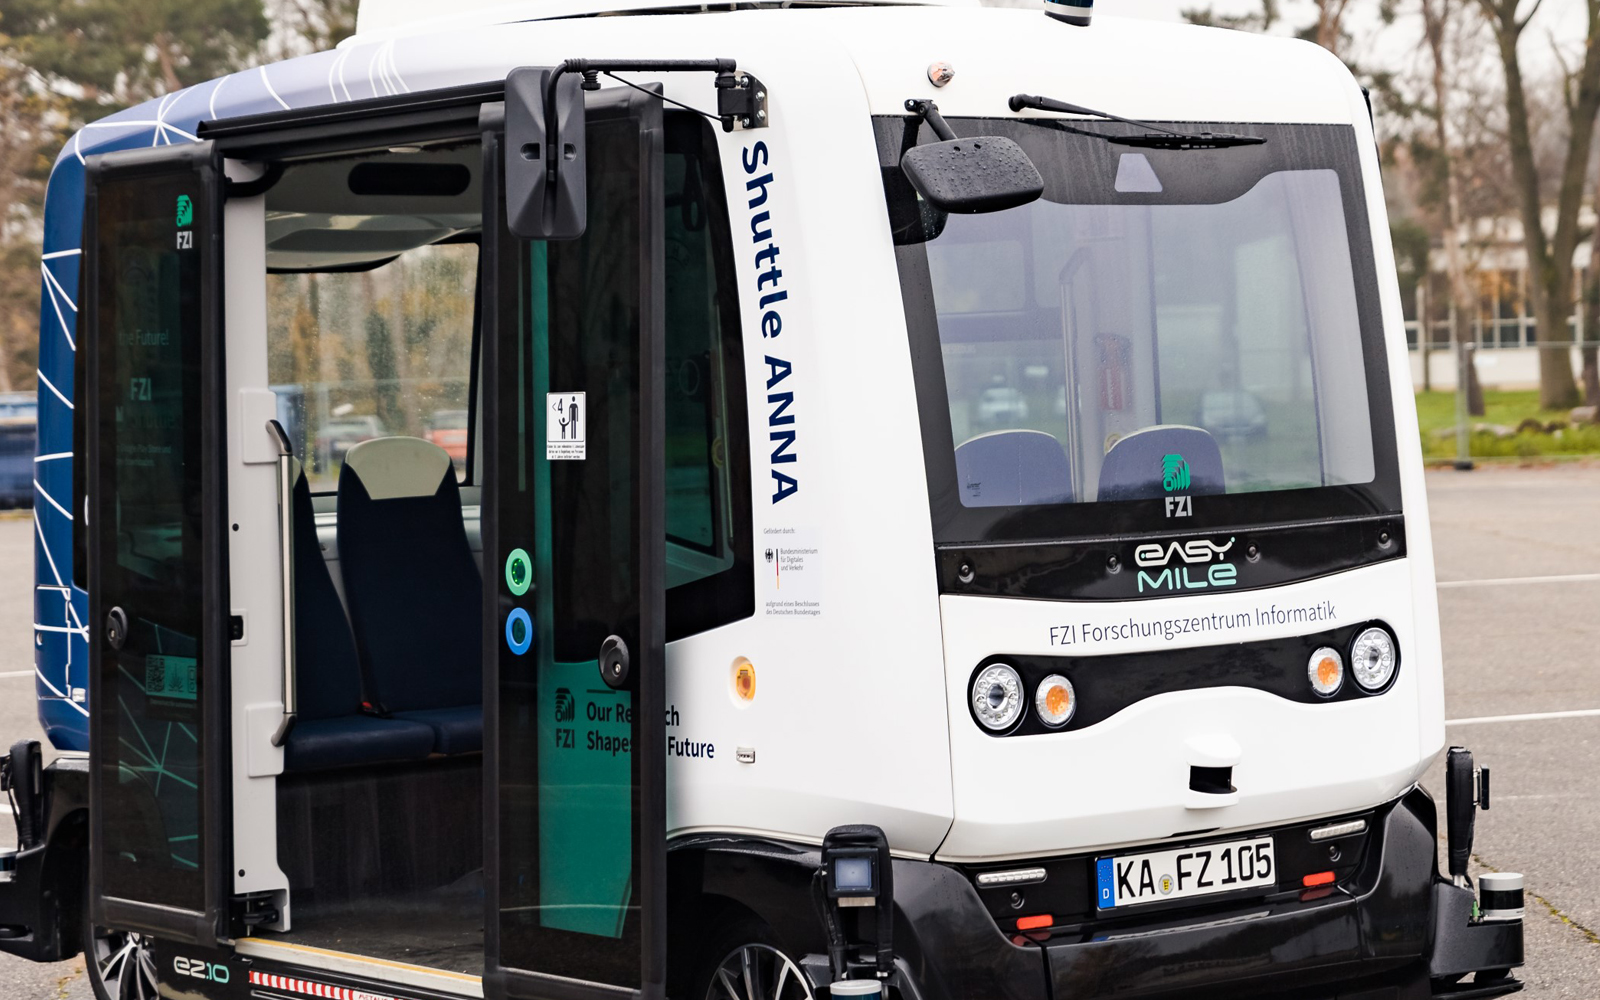
\includegraphics[scale = 0.15]{pictures/Shuttle ganz.jpg}
    \caption{Autonomous FZI shuttle}
    \label{fig:Shuttle}
\end{figure}
Referenz zu Shuttle \ref{fig:Shuttle}
\newpage

% ********************************
% ** Section about the datasets **
% ********************************

\section{dataset comparison}
We concentrated on two different datasets and in the following there will be a short comparison between the two and then there will be a in-detph review of the datasets.

\begin{table}[htbp]
\centering
\begin{tabular}{ c | c c }
 Property & AffectNet & EMOTIC \\ 
\hline
 Train Images & 287651? & 23266? \\
 Validation Images & 3999? & 3315 \\
 Test Images & 0 & 7203 \\
 Emotion Categories & 8? & 26? \\
 VAD & VA & VAD \\
 scaling & -1 to 1 (floats) & 1 to 10 (ints) \\
\end{tabular}
\caption{Comparison of Dataset Properties: AffectNet vs. Emotic}
\label{tab:dataset_properties}
\end{table}


\subsection{AffectNet}
...

\subsection{EMOTions In Context (EMOTIC)}
...

% ********************************
% * Section about model training *
% ********************************
\newpage
\section{Training a model}

\subsection{Improving the baseline AffectNet model}
Starting with a given baseline model, we evaluate different approaches to improve the overall performance of the model. Therefore, not only the classification of the eight labels but also the regression of the continuous values Valence and Aroual is now considered. Hence our overall model performance rating is based on a combination of the state-of-the-art binary classification metrics Precision, Recall and F1-Score extended with the common regression metrics mean-squared-error (MSE), mean-absolut-error (MAE) and root-mean-squared-error (RSME). Our approaches can be differentiated into:

\begin{itemize}
    \item \textbf{Baseline}: Using the baseline code to train a custom EfficientNet B4 model and evaluate the model to  our defined performance metrics. 
    \item \textbf{New Classification}: This approach uses the provided baseline code and applies the proposed improvement methodologies, such as a weighted CrossEntropyLoss. As proposed in the baseline code, we stick to the usage of a custom EfficientNet B4 model. 
    \item \textbf{Regression (Val \& Aro)}: With this approach, we change the model structure and our loss function to predict only the two continuous values Valence and Arousal using a MSELoss.
\item \textbf{Combined}: This approach combines the new classification approach with the regression approach. To achive this, the model strucutre is extended to have ten output neurons, splitted in eight classification neurons and two regression neurons. Hence the overall loss is calculated using the sum of the weighted CrossEntropyLoss and the MSELoss.
\item \textbf{Priori Knowledge}: Using the given knowledge of the true labels for each image, our model knows the label and predicts the two continuous values Valence and Arousal. Therefore, the fully connected layer model is extended, such that the feature extraction is only applied to the image and the classification depends also on the given class labels.
\item \textbf{Two Sequential Models}: First, we use the classification model to predict the true label of each image. Using this prediction, our second model - similar to the priori knowledge approach - uses the image and the label knowledge to predict the values Valence and Arousal.
\end{itemize}





\newpage

\begin{table}[htbp]
\centering
\rotatebox{90}{
\begin{tabular}{c | c c c c c c}
 Approach & Precision & Recall & F1-Score & MSE & MAE & RMSE \\ 
 \hline
 Baseline & & & & & & \\
 \hline
 New Classification & & & & & & \\
 \hline
 Regression (Val \& Aro) & & & & & & \\
 \hline
 Combined & & & & & & \\
 \hline
 Priori Knowledge & & & & & & \\
 \hline
 Two sequential models & & & & & & \\
 \hline
\end{tabular}
}
\caption{Performance Metrics Comparison for Various Approaches}
\label{tab:metrics}
\end{table}

Our best approach is reached using the following hyperparameters ...

\begin{table}[htbp]
\centering
\begin{tabular}{c | c }
 Hyperparameter & Choosen \\ 
  \hline
 Batch Size & 64 \\
 \hline
 LR & 4e-5 \\
 \hline
  Optimizer & AdamW \\
 \hline
 Loss functions & Weighted CrossEntropyLoss, MSELoss \\
 \hline
 Scheduler & CosineAnnealingLR \\
\end{tabular}
\caption{Selected Hyperparameters for the Model}
\label{tab:hyperparameters}
\end{table}

\newpage
\subsection{Applying our training methodology to the EMOTIC dataset}


\newpage
\bibliographystyle{IEEEtran}  % Choose the IEEEtran bibliography style
\bibliography{literature.bib}  % Specify the name of your .bib file without the extension



\end{document}
